% Meta-Informationen -------------------------------------------------------
%		Informationen über das Dokument, wie z.B. Titel, Autor, Matrikelnr. etc
%		werden in der Datei _Meta.tex definiert und können danach global
%		verwendet werden.
% --------------------------------------------------------------------------
% Informationen ------------------------------------------------------------
% 	Definition von globalen Parametern, die im gesamten Dokument verwendet
% 	werden können (z.B auf dem Deckblatt etc.).
% --------------------------------------------------------------------------
\newcommand{\titel}{Exposé\\Federated Learning With Individualized Differential Privacy}
\newcommand{\art}{Master's Thesis} %Bachelorarbeit
\newcommand{\ort}{Leipzig}
\newcommand{\hochschule}{Leipzig University}
\newcommand{\fachgebiet}{Database Group}
\newcommand{\fakultaet}{Faculty of Mathematics and Computer Science}
\newcommand{\institut}{Department of Computer Science}
\newcommand{\autor}{Ole Borchardt}
\newcommand{\matrikelnr}{3725924}
\newcommand{\erstbetreuer}{Prof. Dr. Erhard Rahm}
\newcommand{\zweitbetreuer}{XXXXX}
\newcommand{\jahr}{2024}
\newcommand{\invnr}{1337}
\newcommand{\eingereicht}{xx.xx.xxxx}

% Eigene Befehle
\newcommand{\todo}[1]{\textbf{\textsc{\textcolor{red}{(TODO: #1)}}}}

% Autorennamen in small caps
\newcommand{\AutorZ}[1]{\textsc{#1}}
\newcommand{\Autor}[1]{\AutorZ{\citeauthor{#1}}}

% Befehle zur semantischen Auszeichnung von Text
\newcommand{\NeuerBegriff}[1]{\textbf{#1}}
\newcommand{\Fachbegriff}[1]{\textit{#1}}
\newcommand{\Prozess}[1]{\textit{#1}}
\newcommand{\Webservice}[1]{\textit{#1}}
\newcommand{\Eingabe}[1]{\texttt{#1}}
\newcommand{\Code}[1]{\texttt{#1}}
\newcommand{\Datei}[1]{\texttt{#1}}
\newcommand{\Datentyp}[1]{\textsf{#1}}
\newcommand{\XMLElement}[1]{\textsf{#1}}

% Abkürzungen
\newcommand{\vgl}{Vgl.\ }
\newcommand{\ua}{\mbox{u.\,a.\ }}
\newcommand{\zB}{\mbox{z.\,B.\ }}
\newcommand{\bs}{$\backslash$}

% Einfache Anführungszeichen in texttt
\newcommand{\sq}{\textquotesingle}



% Dokumentenkopf -----------------------------------------------------------
% 	Diese Vorlage basiert auf "scrreprt" aus dem koma-script.
%		Die Option draft sollte beim fertigen Dokument ausgeschaltet werden.
% --------------------------------------------------------------------------
\documentclass[
	11pt,					% Schriftgröße
	DIV=10,
	ngerman,				% für Umlaute, Silbentrennung etc.
	a4paper,				% Papierformat
	oneside,				% einseitiges Dokument
	titlepage,				% es wird eine Titelseite verwendet
	parskip=half,			% Abstand zwischen Absätzen (halbe Zeile)
	headings=normal, % Größe der Überschriften verkleinern
	numbers=withendperiod, % Fügt in den Überschriften nach den Zahlen einen Punkt ein
	listof=totoc,				% Verzeichnisse im Inhaltsverzeichnis aufführen
	bibliography=totoc,				% Literaturverzeichnis im Inhaltsverzeichnis aufführen
	index=totoc,				% Index im Inhaltsverzeichnis aufführen
	captions=tableheading,		% Beschriftung von Tabellen oberhalb ausgeben
	final					% Status des Dokuments (final/draft)
]{scrreprt}

\renewcommand*\chapterheadstartvskip{\vspace*{-1.0cm}}

% Bentigte Packages -------------------------------------------------------
%		Weitere Packages, die benötigt werden, sind in die Datei Packages.tex
%		"ausgelagert", um die Vorlage möglichst übersichtlich zu halten.
% --------------------------------------------------------------------------
% Anpassung des Seitenlayouts ----------------------------------------------
% 	siehe Seitenstil.tex
% --------------------------------------------------------------------------
\usepackage[
	automark,			% Kapitelangaben in Kopfzeile automatisch erstellen
	headsepline,	% Trennlinie unter Kopfzeile
	ilines				% Trennlinie linksbündig ausrichten
]{scrlayer-scrpage}
\usepackage{scrhack} % Disable some warnings

\usepackage{pseudocode}
\usepackage{nicefrac}

% Für eine schöne Anordnung von Bildern
%\usepackage{subfigure}

\usepackage{dsfont}
%\usepackage{color}
%
%% Define user colors using the RGB model
%\definecolor{yellow}{rgb}{0.0,1.0,0.0}
%\definecolor{rot}{rgb}{1.0,0.0,0.0}

% Anpassung an Landessprache -----------------------------------------------
% 	Verwendet globale Option german siehe \documentclass
% --------------------------------------------------------------------------
\usepackage[ngerman]{babel}

% Umlaute ------------------------------------------------------------------
% 		Umlaute/Sonderzeichen wie äöüß direkt im Quelltext verwenden (CodePage).
%		Erlaubt automatische Trennung von Worten mit Umlauten.
% --------------------------------------------------------------------------
\usepackage[utf8]{inputenc}
%\usepackage[T1]{fontenc}
%\usepackage{ae} % "schöneres" ä
\usepackage{textcomp} % Euro-Zeichen etc.
\usepackage{lmodern} % schööön

% Grafiken -----------------------------------------------------------------
% 		Einbinden von Grafiken [draft oder final]
% 		Option [draft] bindet Bilder nicht ein - auch globale Option
% --------------------------------------------------------------------------
\usepackage[dvips,final]{graphicx}
\usepackage{wrapfig}
\graphicspath{{Bilder/}} % Dort liegen die Bilder des Dokuments

% Befehle aus AMSTeX für mathematische Symbole z.B. \boldsymbol \mathbb ----
\usepackage{amsmath,amsfonts,amsthm}

% Für Index-Ausgabe; \printindex -------------------------------------------
\usepackage{makeidx}

% Einfache Definition der Zeilenabstände und Seitenränder etc. -------------
\usepackage{setspace}
\usepackage{geometry}

% für gedrehte Tabellen
\usepackage{rotating} 

% Symbolverzeichnis --------------------------------------------------------
% 	Symbolverzeichnisse bequem erstellen, beruht auf MakeIndex.
% 		makeindex.exe %Name%.nlo -s nomencl.ist -o %Name%.nls
% 	erzeugt dann das Verzeichnis. Dieser Befehl kann z.B. im TeXnicCenter
%		als Postprozessor eingetragen werden, damit er nicht ständig manuell
%		ausgeführt werden muss.
%		Die Definitionen sind ausgegliedert in die Datei Abkuerzungen.tex.
% --------------------------------------------------------------------------
\usepackage[intoc]{nomencl}
  \let\abbrev\nomenclature
  \renewcommand{\nomname}{Abkürzungsverzeichnis}
  \setlength{\nomlabelwidth}{.25\hsize}
  \renewcommand{\nomlabel}[1]{#1 \dotfill}
  \setlength{\nomitemsep}{-\parsep}

% Zum Umfließen von Bildern -------------------------------------------------
\usepackage{floatflt}

% Zum Einbinden von Programmcode --------------------------------------------
\usepackage{listings}
\usepackage{xcolor} 
\definecolor{hellgelb}{rgb}{1,1,0.9}
\definecolor{colKeys}{rgb}{0,0,1}
\definecolor{colIdentifier}{rgb}{0,0,0}
\definecolor{colComments}{rgb}{1,0,0}
\definecolor{colString}{rgb}{0,0.5,0}
\lstset{%
    float=hbp,%
    basicstyle=\texttt\small, %
    identifierstyle=\color{colIdentifier}, %
    keywordstyle=\color{colKeys}, %
    stringstyle=\color{colString}, %
    commentstyle=\color{colComments}, %
    columns=flexible, %
    tabsize=2, %
    frame=single, %
    extendedchars=true, %
    showspaces=false, %
    showstringspaces=false, %
    numbers=left, %
    numberstyle=\tiny, %
    breaklines=true, %
    backgroundcolor=\color{hellgelb}, %
    breakautoindent=true, %
%    captionpos=b%
}

% Lange URLs umbrechen etc. -------------------------------------------------
\usepackage{url}


%% Wichtig für korrekte Zitierweise ------------------------------------------

\usepackage[autocite=inline, sorting=none, backend=biber]{biblatex}
\addbibresource{quellen.bib} % Name der .bib-Datei

\usepackage{csquotes} % Empfohlen, um Zitierten Text richtig darzustellen

% ermöglicht Zeilenumbrüche in Captions
\usepackage{caption}


% PDF-Optionen --------------------------------------------------------------
\usepackage[
bookmarks,
bookmarksopen=true,
pdftitle={\titel},
pdfauthor={\autor},
pdfcreator={\autor},
pdfsubject={\titel},
pdfkeywords={\titel},
colorlinks=true,
%linkcolor=red, % einfache interne Verknüpfungen
%anchorcolor=black,% Ankertext
%citecolor=blue, % Verweise auf Literaturverzeichniseinträge im Text
%filecolor=magenta, % Verknüpfungen, die lokale Dateien öffnen
%menucolor=red, % Acrobat-Menüpunkte
%urlcolor=cyan, 
% für die Druckversion können die Farben ausgeschaltet werden:
linkcolor=black, % einfache interne Verknüpfungen
anchorcolor=black,% Ankertext
citecolor=black, % Verweise auf Literaturverzeichniseinträge im Text5
filecolor=black, % Verknüpfungen, die lokale Dateien öffnen
menucolor=black, % Acrobat-Menüpunkte
urlcolor=black, 
%backref,
%pagebackref,
plainpages=false,% zur korrekten Erstellung der Bookmarks
pdfpagelabels,% zur korrekten Erstellung der Bookmarks
hypertexnames=false,% zur korrekten Erstellung der Bookmarks
linktocpage % Seitenzahlen anstatt Text im Inhaltsverzeichnis verlinken
]{hyperref}

% Zum fortlaufenden Durchnummerieren der Fußnoten ---------------------------
\usepackage{chngcntr}


% für lange Tabellen
\usepackage{longtable}
\usepackage{array}
\usepackage{ragged2e}
\usepackage{lscape}

\usepackage{supertabular}

% Spaltendefinition rechtsbündig mit definierter Breite ---------------------
\newcolumntype{w}[1]{>{\raggedleft\hspace{0pt}}p{#1}}

% Formatierung von Listen ändern
\usepackage{paralist}
% Standardeinstellungen:
% \setdefaultleftmargin{2.5em}{2.2em}{1.87em}{1.7em}{1em}{1em}

\usepackage{tablefootnote}
% für Ausblenden der Seitenzahl
\usepackage{lipsum}

% für subfigures
\usepackage{caption}
\usepackage{subcaption}

% für Durchschnittszeichen
\usepackage{wasysym}

% für tabellen
\usepackage{multirow}

% Erstellung eines Index und Abkürzungsverzeichnisses aktivieren -----------
\makeindex
% makeindex Masterarbeit.nlo -s nomencl.ist -o Masterarbeit.nls
\makenomenclature


% Kopf- und Fußzeilen, Seitenränder etc. -----------------------------------
% Zeilenabstand ------------------------------------------------------------
\onehalfspacing 
% \setstretch{1,5}

% Seitenränder -------------------------------------------------------------
\geometry{paper=a4paper,left=25mm,right=20mm,top=20mm, bottom=25mm}
% Notfall maße :)
%\geometry{paper=a4paper,left=35mm,right=25mm,top=25mm, bottom=25mm}



% Kopf- und Fußzeilen ------------------------------------------------------
\pagestyle{scrheadings}

% Kopf- und Fußzeile auch auf Kapitelanfangsseiten -------------------------
\renewcommand*{\chapterpagestyle}{scrheadings}

% Schriftform der Kopfzeile ------------------------------------------------
\renewcommand{\headfont}{\normalfont}

% Kopfzeile ----------------------------------------------------------------
\ihead{\textit{\headmark}}
\chead{}
%\ohead{\includegraphics[scale=1]{Bilder/logoKlein.JPG}}
\ohead{}
\setlength{\headheight}{8mm} % Höhe der Kopfzeile
\setheadwidth[0pt]{textwithmarginpar} % Kopfzeile über den Text hinaus verbreitern

% Fußzeile -----------------------------------------------------------------
% \ifoot{\copyright\ \autor \\ \invnr}
% \ifoot{\copyright\ \autor \\ \matrikelnr}
\ifoot{\autor \\ \matrikelnr}
\cfoot{}
\ofoot{\pagemark}
\setlength{\footskip}{12mm}
\setfootwidth[0pt]{text}

% Überschriften ------------------------------------------------------------
\renewcommand*\chapterheadstartvskip{\vspace*{-0.5cm}} % Platz vor einer Überschrift eines neuen Kapitels


% erzeugt ein wenig mehr Platz hinter einem Punkt --------------------------
\frenchspacing

% Schusterjungen und Hurenkinder vermeiden
\clubpenalty = 10000
\widowpenalty = 10000 
\displaywidowpenalty = 10000


% Quellcode-Ausgabe formatieren --------------------------------------------
%\lstset{numbers=left, numberstyle=\tiny, numbersep=5pt, breaklines=true}
%\lstset{emph={square}, emphstyle=\color{red}, emph={[2]root,base}, emphstyle={[2]\color{blue}}}

\definecolor{gray}{rgb}{0.9,0.9,0.9}

\lstset{%
		basicstyle=\small\ttfamily,language={[LaTeX]TeX},
		numbersep=5mm, 
		numbers=left,
		numberstyle=\tiny,
		breaklines=true,
		framexleftmargin=8mm, 
		xleftmargin=8mm,
		backgroundcolor=\color{gray},
		captionpos=b
}%

% Fußnoten fortlaufend durchnummerieren ------------------------------------
\counterwithout{footnote}{chapter}

% Definitionen

\newtheorem{definition}{Definition}


% Eigene Definitionen für Silbentrennung
\hyphenation{Trenn-bar-es}
\hyphenation{Al-go-rith-mus}
\hyphenation{DP-Al-go-rith-men}
% Das eigentliche Dokument -------------------------------------------------
%		Der eigentliche Inhalt des Dokuments beginnt hier. Die einzelnen Seiten
%		und Kapitel werden in eigene Dateien ausgelagert und hier nur inkludiert.
% --------------------------------------------------------------------------

\begin{document}
% auch subsubsection nummerieren
\setcounter{secnumdepth}{3}
\setcounter{tocdepth}{3}

% keine Kopf-/Fußzeilen bei Deckblatt und Abstract
\ofoot{}
% Deckblatt
\thispagestyle{plain}
\begin{titlepage}

\begin{center}

\includegraphics[height=7cm]{Bilder/Uni-L.png}\\[2.5ex]

\institut\\
\fakultaet\\
\fachgebiet\\[6ex]

\textbf{\large\titel}\\[1.5ex]
\art\\[6ex]

\normalsize
vorgelegt von:\\
\autor\\[1.5ex]
Matrikelnummer:\\
\matrikelnr\\[1.5ex]
Betreuer:\\
\erstbetreuer\\
\zweitbetreuer\\[1.0ex]
\end{center}

%\begin{tabbing}
%\hspace{3.5cm}\= \kill
%   vorgelegt von: \> \autor\\[1.2ex]
%   Matrikelnummer: \> \matrikelnr\\[1.2ex]
%    \> \\
%   Betreuer: \> \erstbetreuer\\[1.2ex]
%    \> \zweitbetreuer
%\end{tabbing}

\begin{center}
\copyright\ \jahr\\[1.0ex]
\end{center}

\singlespacing
\small
\noindent Dieses Werk einschließlich seiner Teile ist \textbf{urheberrechtlich geschützt}. Jede Verwertung außerhalb der engen Grenzen des Urheberrechtgesetzes ist ohne Zustimmung des Autors unzulässig und strafbar. Das gilt insbesondere für Vervielfältigungen, Übersetzungen, Mikroverfilmungen sowie die Einspeicherung und Verarbeitung in elektronischen Systemen.

\end{titlepage}


% \section*{Danksagung}
\label{sec:Danksagung}
Danksagung
\newpage
\ofoot{\pagemark}

% Seitennummerierung -------------------------------------------------------
%		Vor dem Hauptteil werden die Seiten in großen römischen Ziffern 
%		nummeriert...
% --------------------------------------------------------------------------
\pagenumbering{Roman}

%\tableofcontents			% Inhaltsverzeichnis

% Abkürzungsverzeichnis ----------------------------------------------------
%\input{Inhalt/Glossar}
%\printnomenclature
%\label{sec:Glossar}

%\listoffigures					% Abbildungsverzeichnis
%\listoftables					% Tabellenverzeichnis

%\renewcommand{\lstlistlistingname}{Verzeichnis der Listings}
%\lstlistoflistings	

% ...danach in normalen arabischen Ziffern ---------------------------------
\clearpage
\pagenumbering{arabic}


% Inhalt -------------------------------------------------------------------
%		Hier können jetzt die einzelnen Kapitel inkludiert werden. Sie müssen
%		in den entsprechenden .TEX-Dateien vorliegen. Die Dateinamen können
% 		natürlich angepasst werden.
% --------------------------------------------------------------------------
\chapter{Introduction}

Federated learning is a training method in machine learning (ML) in which models are trained locally at the location where the data for the training is generated. This avoids sending sensitive data to a central server and allows models to be further optimised on local data, such as in the case of word prediction for smartphone keyboards \parencite{mcmahan:2018}. 

Despite the decentralised structure, privacy risks remain with Federated Learning. For example, federated learning cannot prevent membership inference attacks. Differential Privacy (DP), on the other hand, can very well prevent them \parencite{shokri:2017}. 

However, the use of DP leads to a utility-privacy trade-off. Although \textcite{mcmahan:2018} has shown that accuracy can be maintained even under DP guarantees, this comes at the price of significantly more computational effort. Individual privacy budgets can help to minimise the loss of \textit{utility}. With classic DP training algorithms, the same privacy requirement is applied to all data. As different people have different privacy requirements for their data in reality, the strictest requirements are unnecessarily strict for a large proportion of the data. This can significantly impair the utility, i.e. the ability to learn from the data. In order to better reflect this heterogeneity in the requirements, research is being conducted into algorithms that optimally utilise these heterogeneous privacy budgets.

The aim of this work is to develop and evaluate a training algorithm in a federated learning scenario, taking individual privacy budgets into account. In this scenario the clients have individual privacy budgets for their training data. The aim is not to protect the clients from the aggregating server, but to obtain a model at the end of the training process that complies with the individual privacy budgets.

\section{Differential Privacy}

Differential privacy is a concept for maintaining privacy when processing sensitive data that was introduced by \textcite{dwork:2006}. In principle, noise is added to query results in order to guarantee that the query result would occur with a similar probability for a \textit{adjacent data set}. This guarantees that the influence of a single data point on the query result is limited. The similarity of the probabilities is determined by the \textit{privacy budget} $\epsilon$. A less strict, but in practice much used definition also introduces a $\delta \in [0,1]$, which provides a probability that no privacy guarantees are observed. In \textcite{abadi:2016}, differential privacy is defined as follows:

\begin{definition}
  \emph{\textbf{$(\epsilon, \delta)$-Differential Privacy}} A \textit{randomized mechanism} $\mathcal{M}: \mathcal{D} \rightarrow \mathcal{R}$ with domain $\mathcal{D}$ and range $\mathcal{R}$ satisfies $(\epsilon, \delta)$-differential privacy if for any two adjacent inputs $d$, $d' \in \mathcal{D}$ and for any subset of outputs $S \subseteq \mathcal{R}$ it holds that $$\Pr[\mathcal{M}(d) \in S] \leq e^{\epsilon} \Pr[\mathcal{M}(d') \in S] + \delta$$
\end{definition}

Based on this definition, there are further theorems that enable the development of more complex DP algorithms. The first is the \textit{post processing} theorem. It states that the further processing of data from a DP mechanism cannot further increase the loss of privacy. This property is important, for example, in order to be able to use models trained with privacy guarantees after training without hesitation. In addition, there are composition theorems that provide estimates for the fact that data is processed multiple times.

Noise is added using various mechanisms. Random values are drawn from distributions for which it has been proven that they fulfil the definition of differential privacy. For numerical queries, there is the Laplace mechanism, which draws the random values from the Laplace distribution, and the Gaussian mechanism, which draws the random values from the normal distribution. The Exponential Mechanism, for example, is suitable for categorical queries. Further details are described by \textcite{chang:2023}.

Since the strength of the added noise should be proportional to the greatest possible influence of a data point on the query result, it is also often necessary to limit the value range \parencite[p.31]{chang:2023}. For count queries, this influence is naturally limited to $1$, but if for example an average salary is requested, it is necessary to define the value range of the possible salaries. The greatest possible influence of a data point is called \textit{sensitivity}.


\chapter{Differential Privacy in Machine Learning}

Machine learning models can also be regarded as queries on a data set. A DP mechanism can be applied to them at different points in time, as can be seen in \autoref{fig:design_principles_dpml}. Adding noise in the respective steps has various advantages and disadvantages.

\begin{figure}[tb]
  \centering
  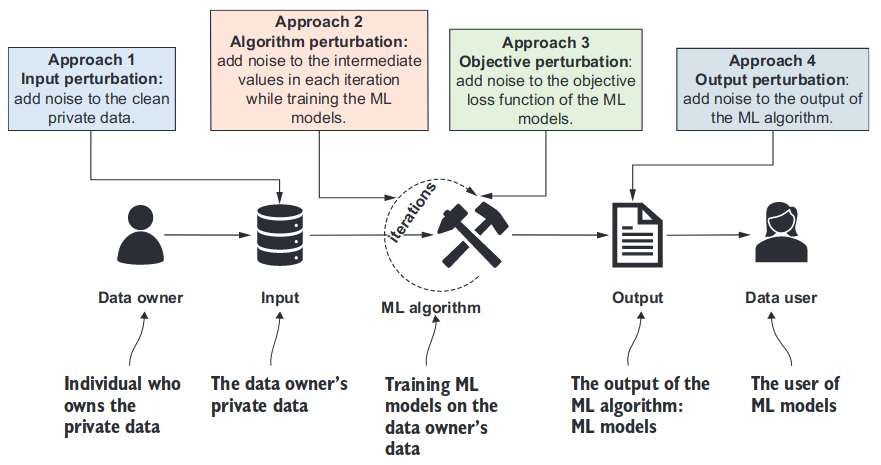
\includegraphics[width=0.7\textwidth]{Bilder/design_principles_dpml.png}
  \caption{Design principles of differentially private ML from \textcite{chang:2023}}
  \label{fig:design_principles_dpml}
\end{figure}

With \textit{input pertubation}, noise is added to the training data before training. This is easy to implement and versatile, but also requires a larger amount of noise as the data usually has a high \textit{sensitivity}.

Using \textit{algorithm pertubation}, the models are trained with unchanged data. In iterative algorithms, the intermediate results can be distorted in the individual steps. \textcite{abadi:2016}, for example, add noise to the gradients.

\textit{Output pertubation} adds noise to the outputs generated by the model. However, the method is not applicable if the model is to be published, as the number of requests to the model cannot be predicted and therefore no privacy guarantees are possible.

With \textit{Objective pertubation}, noise is added to the \textit{Objective function} for which the model is optimised.

The Differentially Private-Stochastic Gradient Descent (DP-SGD) presented by \textcite{abadi:2016} is now a widely used algorithm for training neural networks, on which many other works are based. It is based on the \textit{Stochastic Gradient Descent} (SGD), an iterative optimisation algorithm that is used in various machine learning methods. Compared to the SGD, the DP-SGD has some additional hyperparameters to fulfil the privacy guarantees:

\begin{itemize}
  \item \textbf{Noise scale $\sigma$} A factor by which the noise of the DP mechanism is controlled. 
  \item \textbf{Lot size $L$} The number of data points that are included in a gradient update.
  \item \textbf{Gradient norm bound $C$} All calculated gradients are clipped so that they have a maximum $\ell_2$ norm of $C$. This is necessary because noise with the Gaussian mechanism is added in the following and the sensitivity of vectors is defined via the $\ell_2$ norm. 
\end{itemize}

During training, these parameters affect how quickly a desired $(\epsilon, \delta)$ privacy budget is exhausted. In their results, \textcite{abadi:2016} show that the choice of these parameters (in addition to the parameters from the normal SGD) also has an effect on the accuracy of the model under a fixed privacy budget.

In addition to the specific algorithm, \textcite{abadi:2016} developed the \textit{Moments Accountant}, a method for estimating the loss of privacy during training, which is asympotically much more accurate than classical estimates using composition theorems. They prove this benefit in their work through empirical experiments.

In their paper, \textcite{mcmahan:2018} develop a variant of the \textit{Federated Averaging} (FedAvg) algorithm \parencite{mcmahan:2016} based on the work of \textcite{abadi:2016}, which ensures DP guarantees for users. Their goal is to train an LSTM model for \textit{Next-Word Prediction} on mobile devices. They transfer the definition of adjacent datasets to federated learning by defining the neighbourhood by adding or removing all data of a user. In their experiments, they show that the accuracy of the model can be maintained under DP guarantees, but at a higher computational cost.

The main changes compared to the non-private FedAvg are a limited sensitivity at the clients (by clipping) and at the server (by estimators of the aggregation with a limited range of values). In addition, the server adds noise to the aggregated update based on sensitivity.

\section{Differential privacy with heterogeneous privacy budgets}

\textcite{boenisch:2023} show that the assumption of a privacy budget for all data points limits the possibilities of a model to learn from a data set, since the strictest privacy budget must be assumed for all. In reality, however, different users who generate the data have different privacy requirements. They provide two approaches for training with heterogeneous privacy budgets: the first (\textbf{SAMPLE}) utilises the privacy budget of less private data points by drawing them with a higher probability during training. The second approach (\textbf{SCALE}) controls the privacy budget used by individualising the \textit{noise multiplier} and \textit{clipping norms}.

\textcite{aldaghri:2023} present an algorithm to benefit from heterogeneous privacy requirements in federated learning scenarios. Similar to the \textbf{SCALE} algorithm from \textcite{boenisch:2023}, it uses individual noise scales for each group with the same privacy level. In addition, only two gradations of privacy levels are evaluated, namely clients without privacy requirements and clients with privacy requirements. To track the \textit{privacy loss} they use a moments accountant from \textcite{abadi:2016} for each group of cleints with the same privacy requirements.


\chapter{Method}

In this work, the sampling approach of \textcite{boenisch:2023} is to be adapted to a federated learning scenario. It replaces the \textit{poisson sampling} of \textcite{abadi:2016} with a sampling of the data that is dependent on the respective \textit{privacy budget}. As with \textcite{aldaghri:2023} and \textcite{mcmahan:2018}, the aim of my work is to comply with the (heterogeneous) DP guarantees in the final model. In particular, the aim is therefore not to protect the clients from the aggregating server during training.

To ensure compliance, like \textcite{boenisch:2023} and \textcite{aldaghri:2023}, I will use a \textit{moments accountant} for each group with the same privacy budget. In addition, I will use the \textit{FedAvg} algorithm, which is also the basis for \textcite{aldaghri:2023}.

The following questions will be important in the course of my work: How can I monitor the privacy loss of each client during training? How can I aggregate the clipped gradients of the clients on the server? Can the implementation of \textcite{boenisch:2023} for calculating the sample probabilities of individual data points be transferred to the clients in the federated learning scenario? Does the use of individual privacy budgets with my algorithm have advantages over algorithms with homogeneous privacy budgets?

\section{Implementation}

The implementation is possible with both Pytorch and Tensorflow. With Pytorch, Flower \parencite{beutel:2020} for federated learning and Opacus \parencite{yousefpour:2021} for the privacy guarantees would be suitable. Opacus is a good choice, as \textcite{boenisch:2023} have provided their implementation, which is based on Opacus. However, Opacus is more experimental than the Tensorflow libraries, as technical bugs\footnote{\url{https://github.com/pytorch/opacus/issues/612}, accessed: 2024-03-08}, for example, have not yet been fixed in the current release (as of March 2024). 

Tensorflow, on the other hand, offers a module for Differential Privacy \parencite{tfprivacy} as well as for Federated Learning \parencite{tffederated}. In particular, the use of both modules together is very well documented compared to the Pytorch libraries. In addition, relevant parts of the implementation of \textcite{boenisch:2023} can also be transferred to the Tensorflow ecosystem using Google's differential privacy library \parencite{googledp}.

For the reasons mentioned, I will first try to implement the algorithms in my work with Tensorflow. Apart from that, I will work on the Leipzig University cluster\footnote{\url{https://www.sc.uni-leipzig.de/}, accessed: 2024-03-11} and use Docker containers for reproducibility. I will store both the containers and my code in a GitHub repository.

\section{Evaluation}
The evaluation of my approach should cover two areas in particular: On the one hand, compliance with the privacy guarantees for the respective clients, and on the other hand, the potential gain in utility for the trained model. The latter can be evaluated using common metrics such as accuracy, precision, recall, AUC or computational effort. The upper performance limit would be a non-private model, the lower one a model that is trained in compliance with the privacy guarantees of the strictest group.

In my opinion, checking compliance with the privacy guarantees is the greater challenge. \textcite{aldaghri:2023} only examine these theoretically. \textcite{boenisch:2023} evaluate their approach with regard to membership inference attacks. This is also the aim of my work. In addition, the accountants can be used to verify at which points in time the budgets of the individual clients are exhausted. In particular, my algorithm should prevent the privacy budgets of the stricter clients from being exhausted more quickly.




%\include{Inhalt/Grundlagen...}

% Literaturverzeichnis -----------------------------------------------------
%		Das Literaturverzeichnis wird aus der Datenbank erstellt.
%		Die genaue Verwendung von biblatex wird hier jedoch nicht erklärt.
%		Links: 	https://ctan.org/pkg/biblatex?lang=de
%						https://de.overleaf.com/learn/latex/Articles/Getting_started_with_BibLaTeX
% --------------------------------------------------------------------------

\printbibliography

% \setcounter{page}{122}
% \pagenumbering{gobble}
% %\pagenumbering{gobble}
\addchap{Erklärung}
Ich versichere, dass ich die vorliegende Arbeit mit dem Thema:

\begin{center}
\textit{\glqq\titel\grqq}\\[1em]
\end{center}
			
selbständig und nur unter Verwendung der angegebenen Quellen und Hilfsmittel angefertigt habe, insbesondere sind wörtliche oder sinngemäße Zitate als solche gekennzeichnet. Mir ist bekannt, dass Zuwiderhandlung auch nachträglich zur Aberkennung des Abschlusses führen kann. Ich versichere, dass das elektronische Exemplar mit den gedruckten Exemplaren übereinstimmt.
\par
\ort, den \eingereicht


\rule[-0.2cm]{5cm}{0.5pt}

\textsc{\autor} 
	% Selbständigkeitserklärung 

% Anhang -------------------------------------------------------------------
%		Die Inhalte des Anhangs werden analog zu den Kapiteln inkludiert.
%		Dies geschieht in der Datei Anhang.tex
% --------------------------------------------------------------------------
%\appendix
%\clearpage
%\renewcommand*{\thesection}{\Alph{section}} 
%\pagenumbering{Roman}
%\include{Inhalt/Anhang}



% Index --------------------------------------------------------------------
%		Zum Erstellen eines Index, die folgende Zeile auskommentieren.
% --------------------------------------------------------------------------
%\printindex		% Index hier einfügen
%\ofoot{}
%\include{Inhalt/Thesen}	% Thesen 

\end{document}
